\documentclass[aspectratio=169]{beamer}
\usetheme{metropolis}

%\usepackage{beamerthemesplit}
%\beamertemplatenavigationsymbolsempty
\usepackage{amsmath}
\usepackage{amsthm}
\usepackage{amssymb}
\usepackage{latexsym}
\usepackage{graphicx}
\usepackage{fancybox}
\usepackage{dsfont}
\usepackage{multirow} 
\usepackage{multicol}
\usepackage{booktabs} 
\usepackage{dcolumn}
\usepackage{soul}
\usepackage[cache=false]{minted}
\renewcommand{\MintedPygmentize}{/Users/christopherconlon/anaconda3/bin/pygmentize}
\usepackage{MnSymbol}
\usepackage{stmaryrd}


\DeclareMathOperator*{\argmax}{arg\,max}
\DeclareMathOperator*{\argmin}{arg\,min}

\newcommand{\X}{\mathtt{X}}
\newcommand{\Y}{\mathtt{Y}}

%\newcommand{\R}{\mathbb{R}}
%\newcommand{\E}{\mathbb{E}}
%\newcommand{\V}{\mathbb{V}}
\newcommand{\p}{\mathbb{P}}
\newcommand*\df{\mathop{}\!\mathrm{d}}
\newcommand{\del}{\partial}


% imports
\usepackage{xargs}
\usepackage{xpatch}
\usepackage{etoolbox}
\usepackage{pdflscape}
\usepackage{booktabs}
\usepackage{threeparttable}
\usepackage[skip=0.2\baselineskip]{caption}

% command for inputting raw latex
\makeatletter
\newcommand\primitiveinput[1]{\@@input #1 }
\makeatother

% common table command
\newcommandx{\tablecontent}[4]{
    \begin{threeparttable}[!ht]
        \centering
        \caption{#3}
        \vspace{-1em}
        \footnotesize
        \begin{tabular}{#1}
            \primitiveinput{../tables/#2.tex}
        \end{tabular}
        \vspace{-0.2em}
        \begin{tablenotes}[flushleft]
            #4
        \end{tablenotes}
    \end{threeparttable}
}




% \usepackage{slashbox}
\title{Lecture 1: Review (Mostly)}
\author{Chris Conlon }
\institute{NYU Stern }


\newcommand{\norm}[1]{\left\lVert#1\right\rVert}
\newcommand{\R}{\mathbb{R}}
\newcommand{\E}{\mathbb{E}}
\newcommand{\V}{\mathbb{V}}
\newcommand{\ol}{\overline}
%\newcommand{\ul}{\underline}
\newcommand{\pp}{{\prime \prime}}
\newcommand{\ppp}{{\prime \prime \prime}}
\newcommand{\policy}{\gamma}


\newcommand{\fp}{\frame[plain]}

\date{\today}

\begin{document}
\maketitle

\begin{frame}[fragile]{Packages for Today}
Let's load some packages so that I can make some better looking plots:\\
\begin{minted}{R}
#always
library(tidyverse)
# for SE's
library(estimatr)
library(broom)
# for Panel
library(lfe)
library(plm)
\end{minted}
\end{frame}


\begin{frame}{Today's Plan}
\begin{itemize}
\item Recap OLS and various forms of standard errors
\item Standard errors are tedious but I guess you are supposed to know this stuff
\item Hopefully first and last time we talk about this
\end{itemize}
\end{frame}


\section{Recap: Asymptotics for OLS and the Linear Model}


\begin{frame}{OLS}
\begin{align*}
y_i = \beta_0 + \beta x_i + u_i
\end{align*}
Recall the three basic OLS assumptions
\begin{enumerate}
\item $E(u_i |X_i ) = 0$
\item $(X_i,Y_i)$, $i =1,\ldots,n$, are i.i.d.
\item Large outliers are rare $E[Y^4]< \infty$ and $E[X^4]<\infty$.
\end{enumerate}
\end{frame}

\begin{frame}{Unbiasedness and Consistency}
\begin{itemize}
\item Unbiasedness means on average we don't over or under estimate $\widehat{\beta}$
\begin{align*}
\E[\widehat{\beta} ] - \beta_0 = 0
\end{align*}
\item Consistency tells us that we approach the true $\beta_0$ as $n \rightarrow \infty$.
\begin{align*}
\widehat{\beta}  \overset{p}{\to} \beta_0
\end{align*}
\item Example: $X_{(1)}$ is unbiased but not consistent for the mean.
\item Example $\frac{n}{n-5} \overline{X}$ is consistent but biased for the mean.
\end{itemize}
\end{frame}


\begin{frame}{Bias Variance Decomposition}
We can decompose any estimator into two components
\begin{eqnarray*}
\underbrace{E[(y- \hat{f}(x))^2]}_{MSE} =\underbrace{\left( E[ \hat{f}(x) - f(x)] \right)^2}_{Bias^2}  +  \underbrace{E \left[ \left(  \hat{f}(x) - E[\hat{f}(x)]  \right)^2 \right]}_{Variance} 
\end{eqnarray*}
\begin{itemize}
\item What minimizes MSE?
\begin{eqnarray*}
f(x_i) = E[Y_i | X_i]  
\end{eqnarray*}
\item In general we face a tradeoff between bias and variance.
\item In OLS we minimize the variance among unbiased estimators assuming that the true $f(x_i)= X_i \beta$ is linear. (But is it?)
\end{itemize}
\end{frame}



\begin{frame}{Outliers and Leverage}
One way to find \alert{outliers} is to calculate the \alert{leverage} of each observation $i$. We begin with the \alert{hat matrix}:
\begin{align*}
P = X  (X'X)^{-1} X'
\end{align*}
and consider the diagonal elements which for some reason are labeled $h_{ii}$
\begin{align*}
h_{ii} = x_i (X'X)^{-1} x_i'
\end{align*}
This tells us how \alert{influential} an observation is in our estimate of $\widehat{\beta}$.\\
Particularly important for $\{0,1\}$ \alert{dummy variables} with uneven groups.
\end{frame}


\begin{frame}{Leave One Out Regression}
\begin{itemize}
\item This is sometimes called the \alert{Jackknife}
\item Sometimes it is helpful to know what would happen if we omitted a single observation $i$
\item Turns out we don't need to run $N$ regressions
\begin{align*}
\widehat{\beta}_{-i} &= (X_{-i}'X_{-i})^{-1} X_{-i}' Y_{-i} \\
&=\widehat{\beta} -  (X 'X)^{-1} x_i  \tilde{u}_i  \quad \mbox{ where } \tilde{u}_i = (1-h_{ii})^{-1}\hat{u}_i
\end{align*}
\item $\tilde{u}_i $ has the interpretation of the \alert{LOO prediction error}.
\item high leverage observations move $\widehat{\beta}$ a lot.
\end{itemize}
You can read more about this in Ch3 of Hansen. [Skip derivation]
\end{frame}

\begin{frame}[fragile]{Leverage and QQ plots}
\begin{minted}{R}
library(car)
fit <- lm(mpg~disp+hp+wt+drat, data=mtcars)

# Assessing Outliers
outlierTest(fit) # Bonferonni p-value for most extreme obs
qqPlot(fit, main="QQ Plot") #qq plot for studentized resid 
leveragePlots(fit) # leverage plots
\end{minted}
\end{frame}

\begin{frame}{Leverage Plot}
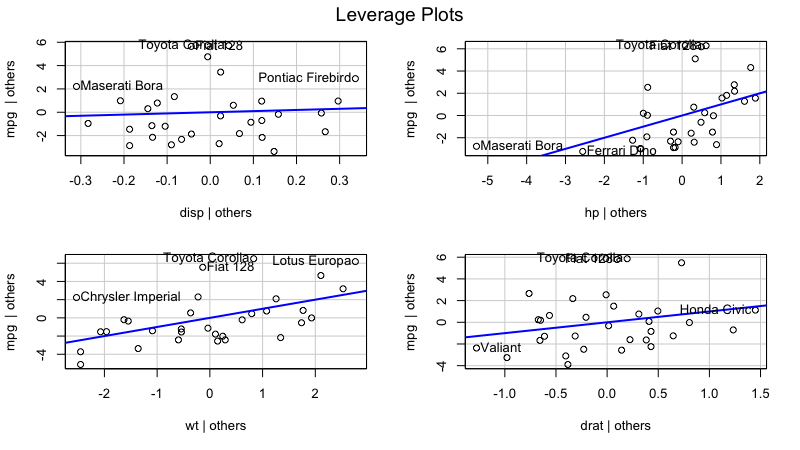
\includegraphics[width=5.5in]{./resources/leverage_plot.png}
\end{frame}




\begin{frame}{Gauss Markov Theorem}
Gauss Markov Adds two assumptions:
\begin{enumerate}
\item $E(u_i |X_i ) = 0$
\item $(X_i,Y_i)$, $i =1,\ldots,n$, are i.i.d.
\item Large outliers are rare $E[Y^4]< \infty$ and $E[X^4]<\infty$.
\item $Var(u_i) = \sigma^2$ (homoskedasticity)
\item $u_i \sim N(0,\sigma^2)$ (normal errors)
\end{enumerate}
Under these assumptions you learned that OLS is \alert{BLUE}
\end{frame}




\begin{frame}{Variance of $\widehat{\beta}$}
Start with the variance of the residuals to form a \alert{diagonal} matrix $D$:
\begin{align*}
\operatorname { Var } ( \mathbf{u} | \mathbf { X } ) &= \mathbb { E } \left( \mathbf{u u} ^ { \prime } | \mathbf { X } \right){ = } \mathbf { D }\\
\mathbf { D } &= \operatorname { diag } \left( \sigma _ { 1 } ^ { 2 } , \ldots , \sigma _ { n } ^ { 2 } \right) = \left( \begin{array} { c c c c } { \sigma _ { 1 } ^ { 2 } } & { 0 } & { \cdots } & { 0 } \\ { 0 } & { \sigma _ { 2 } ^ { 2 } } & { \cdots } & { 0 } \\ { \vdots } & { \vdots } & { \ddots } & { \vdots } \\ { 0 } & { 0 } & { \cdots } & { \sigma _ { n } ^ { 2 } } \end{array} \right)
\end{align*}
\begin{itemize}
\item $\mathbf{D}$ is diagonal because $\mathbb { E }[u_i u_j | X] = \mathbb { E }[u_i  | x_i]  \mathbb { E }[u_j  | x_j]=0$ (independence)
\item The elements of $D_i$ are given by $\mathbb { E }[u_i^2 | X] = \mathbb { E }[u_i^2 | x_i] = \sigma_i^2$.
\item In the \alert{homoskedastic} case $\mathbf{D} = \sigma^2 \mathbf{I}_n$.
\end{itemize}
\end{frame}

\begin{frame}{Variance of $\widehat{\beta}$}
A useful identity for linear algebra:
\begin{align*}
\operatorname { Var } (a \mathbf{Z} ) = a^2 \operatorname { Var }(\mathbf{Z})\\
\operatorname { Var } (A \mathbf{Z} ) = A \operatorname { Var }(\mathbf{Z}) A'
\end{align*}

Recall that $\operatorname { Var } ( \mathbf{Y} |\mathbf{X} )  = \operatorname { Var } ( \mathbf{u} | \mathbf { X } ) $ and also
recall the formula for $\widehat{\beta}$:
\begin{align*}
\widehat{\beta} &= \underbrace{(X'X)^{-1} X' }_{A} Y= A' Y \\
\mathbf{V}_{\widehat{\beta}} = \operatorname { Var }(\widehat{\beta} | X)&= (X'X)^{-1} X'  \operatorname { Var }(Y| X) X (X'X)^{-1} \\
													     &= (X'X)^{-1} (X'  \mathbf{D} X) (X'X)^{-1} 
\end{align*}
We have that $ (X'  \mathbf{D} X)  = \sum_{i=1}^N x_i x_i'\sigma_i^2$. Under homoskedasticity $\mathbf{D} = \sigma^2 \mathbf{I}_n$ and $\mathbf{V}_{\widehat{\beta}} = \sigma^2 (X'X)^{-1}$.
\end{frame}


\begin{frame}{Variance of $\widehat{\beta}$}
\begin{align*}
\mathbf { D } = \operatorname { diag } \left( \sigma _ { 1 } ^ { 2 } , \ldots , \sigma _ { n } ^ { 2 } \right)
= \mathbb { E } \left( u_i u_i'  | \mathbf { X } \right)
= \mathbb { E } \left( \widetilde{\mathbf{D}}| \mathbf { X } \right)
\end{align*}

We can estimate $\widehat{\mathbf{V}}_{\widehat{\beta}}$ by plugging in $\mathbf{D} \rightarrow  \widetilde{\mathbf{D}} $:
\begin{align*}
\mathbf{V}_{\widehat{\beta}} &= (X'X)^{-1} (X'  \widetilde{\mathbf{D}} X) (X'X)^{-1} \\
&= (X'X)^{-1} \left(\sum_{i=1}^N x_i x_i' u_i^2  \right) (X'X)^{-1} 
\end{align*}
The expectation shows us this estimator is unbiased:
\begin{align*}
E[\mathbf{V}_{\widehat{\beta}} | X]
&= (X'X)^{-1} \left(\sum_{i=1}^N x_i x_i' E[u_i^2 | X] \right) (X'X)^{-1} \\
&= (X'X)^{-1} \left(\sum_{i=1}^N x_i x_i' \sigma_i^2 \right) (X'X)^{-1} = (X'X)^{-1} (X' D X) (X'X)^{-1} 
\end{align*}
\end{frame}



\begin{frame}{Heteroskedasticity Consistent (HC) Variance Estimates}
What we need is a consistent estimator for $\hat{u}^2_i$.
\begin{align*}
\mathbf{V}_{\widehat{\beta}}^{HC0}&= (X'X)^{-1} \left(\sum_{i=1}^N x_i x_i' \hat{u}_i^2 \right) (X'X)^{-1} \\
\mathbf{V}_{\widehat{\beta}}^{HC1}&= (X'X)^{-1} \left(\sum_{i=1}^N x_i x_i' \hat{u}_i^2 \right) (X'X)^{-1} \cdot \left(\frac{n}{n-k}  \right)
\end{align*}
Could use leave one out variance estimate:
\begin{align*}
\mathbf{V}_{\widehat{\beta}}^{HC2}&= (X'X)^{-1} \left(\sum_{i=1}^N (1-h_{ii})^{-1} x_i x_i' \hat{u}_i^2 \right) (X'X)^{-1} \\
\mathbf{V}_{\widehat{\beta}}^{HC3}&= (X'X)^{-1} \left(\sum_{i=1}^N (1-h_{ii})^{-2} x_i x_i' \hat{u}_i^2 \right) (X'X)^{-1} \\
\end{align*}
\end{frame}

\begin{frame}{Heteroskedasticity Consistent (HC) Variance Estimates}
\begin{itemize}
\item We know that $\mathbf{V}_{\widehat{\beta}}^{HC3} > \mathbf{V}_{\widehat{\beta}}^{HC2} > \mathbf{V}_{\widehat{\beta}}^{HC0}$ because $(1- h_{ii}) <1$.
\item $HC3$ are the most \alert{conservative} and also place the most weight on potential outliers.
\item \texttt{Stata} uses $HC1$ as the default and it is what most people refer to when they say \alert{robust standard errors}.
\item These are often called White (1980) SE's or Eicher-Huber-White SE's.
\item In small sample some evidence that $HC2$ does better.
\end{itemize}
\end{frame}

\begin{frame}[fragile]{Heteroskedasticity Consistent (HC) Variance Estimates}
\footnotesize
To read about SE's in \texttt{estimatr}:
\url{ https://declaredesign.org/r/estimatr/articles/mathematical-notes.html}
\begin{minted}{R}
dat <- data.frame(X = matrix(rnorm(2000*5), 2000), y = rnorm(2000))
hc0<-lm_robust(y ~ ., data = dat, se_type="HC0")$std.error
hc1<-lm_robust(y ~ ., data = dat, se_type="HC1")$std.error
hc2<-lm_robust(y ~ ., data = dat, se_type="HC2")$std.error
hc3<-lm_robust(y ~ ., data = dat, se_type="HC3")$std.error
all(hc2 > hc0 )
[1] TRUE
all(hc3> hc2 )
[1] TRUE
\end{minted}
\end{frame}

\begin{frame}{What is Clustering?}
Suppose we want to relax our i.i.d. assumption:
\begin{itemize}
\item Each observation $i$ is a \alert{villager} and each group $g$ is a \alert{village}
\item Each observation $i$ is a \alert{student} and each group $g$ is a \alert{class}.
\item Each observation $t$ is a \alert{year} and each entity $i$ is a \alert{state}.
\item Each observation $t$ is a \alert{week} and each entity $i$ is a \alert{shopper}.
\end{itemize}
We might expect that $\operatorname { Cov } (u_{g1},u_{g2},\ldots,u_{gN}) \neq 0 \rightarrow$ independence is a bad assumption. 
\end{frame}

\begin{frame}{Clustering: Intuition}
The groups (villages, classrooms, states) are independent of one another, but within each group we can allow for arbitrary correlation.
\begin{itemize}
\item If correlation is within an individual over time we call it \alert{serial correlation} or \alert{autocorrelation}
\item Just like in time-series$\rightarrow$ we have fewer effective independent observations in our sample.
\item Asymptotics now about the number of groups $G \rightarrow \infty$ not observations $N \rightarrow \infty$
\end{itemize}
\end{frame}

\begin{frame}{Clustering}
Begin by stacking up observations in each group $\mathbf{y}_{g }  = [y_{g1},\ldots,y_{g n_g}]$, we can write OLS three ways:
\begin{align*}
y_{ig } &= x_{ig}' \beta + u_{ig}\\
\mathbf{y}_{g } &= \mathbf{X}_{g} \beta + \mathbf{u}_{g}\\
\mathbf{Y} &= \mathbf{X} \beta + \mathbf{u}
\end{align*}
All of these are equivalent:
\begin{align*}
\widehat {  \beta  } &= \left( \sum _ { g = 1 } ^ { G } \sum _ { i = 1 } ^ { n _ { g } } x _ { i g }' { x } _ { i g } \right) ^ { - 1 } \left( \sum _ { g = 1 } ^ { G } \sum _ { i = 1 } ^ { n _ { g } } x _ { i g }' y _ { i g } \right)\\
\widehat {  \beta  }  &=  \left(  \sum _ { g = 1 } ^ { G } \mathbf{X}_g' \mathbf{X}_g \right)^{-1} \left(  \sum _ { g = 1 } ^ { G } \mathbf{X}_g' \mathbf{y}_g \right)\\
\widehat {  \beta  }  &=  \left( \mathbf{X}' \mathbf{X} \right)^{-1} \left(   \mathbf{X}' \mathbf{Y} \right)\\
\end{align*}
\end{frame}

\begin{frame}{Clustering (Continued)}
The error terms have covariance within each cluster $g$ as:
\begin{align*}
 \boldsymbol{\Sigma}_ { g } = \mathbb { E } \left( \mathbf{u} _ { g }  \mathbf{ u } _ { g } ^ { \prime } | \boldsymbol { X } _ { g } \right)
\end{align*}

In order to calculate $\widehat{V}_{\widehat{\beta}}$ we replace the covariance matrix $\mathbf{D}$ with $\Omega$ and consider an estimator $\widehat{\Omega}_n$. We exploit \alert{independence across clusters}:
\begin{align*}
\operatorname { var } \left( \left( \sum _ { g = 1 } ^ { G } \boldsymbol { X } _ { g } ^ { \prime } \mathbf{u}_ { g } \right) | \boldsymbol { X } \right) = \sum _ { g = 1 } ^ { G } \operatorname { var } \left( \boldsymbol { X } _ { g } ^ { \prime } \boldsymbol { u } _ { g } | \boldsymbol { X } _ { g } \right)
= \sum _ { g = 1 } ^ { G } \boldsymbol { X } _ { g } ^ { \prime } \mathbb { E } \left( \boldsymbol { u } _ { g } \boldsymbol { u } _ { g } ^ { \prime } | \boldsymbol { X } _ { g } \right) \boldsymbol { X } _ { g }
= \sum _ { g = 1 } ^ { G } \boldsymbol { X } _ { g } ^ { \prime } \boldsymbol { \Sigma } _ { g } \mathbf { X } _ { g } 
 \equiv \Omega_N
\end{align*}
And an estimate of the variance:
\begin{align*}
\boldsymbol { V } _ { \widehat { \boldsymbol { \beta } } } = \operatorname { var } ( \widehat { \boldsymbol { \beta } } | \boldsymbol { X } )
= \left( \mathbf { X } ^ { \prime } \mathbf { X } \right) ^ { - 1 } \boldsymbol { \Omega } _ { n } \left( \mathbf { X } ^ { \prime } \mathbf { X } \right) ^ { - 1 }
\end{align*}
\end{frame}


\begin{frame}{Clustered SE's}
\begin{align*}
\widehat { \Omega } _ { n } &= \sum _ { g = 1 } ^ { G } X _ { g } ^ { \prime } \widehat {\mathbf{ u }} _ { g }\widehat {\mathbf{ u }}_{g} ^ { \prime } X _ { g }\\
&= \sum _ { g = 1 } ^ { G } \sum _ { i = 1 } ^ { n _ { g } } \sum _ { \ell = 1 } ^ { n _ { g } } x _ { i g } x _ { \ell g } ^ { \prime } \widehat { u } _ { i g } \widehat { u } _ { \ell g }\\
&= \sum _ { g = 1 } ^ { G } \left( \sum _ { i = 1 } ^ { n _ { g } } x _ { i g } \widehat { u } _ { i g } \right) \left( \sum _ { \ell = 1 } ^ { n _ { g } } x _ { \ell g } \widehat { u } _ { \ell g } \right) ^ { \prime }
\end{align*}
\begin{itemize}
\item First line makes explicit: independence over each of $G$ clusters
\item Last line easiest for computer
\end{itemize}
\end{frame}

\begin{frame}{Clustered SE's}
\begin{align*}
\widehat { \boldsymbol { V } } _ { \hat { \beta } } ^ { \mathrm { CR } 1 } = \left( \boldsymbol { X } ^ { \prime } \boldsymbol { X } \right) ^ { - 1 } \left( \sum _ { g = 1 } ^ { G } \boldsymbol { X } _ { g } ^ { \prime } \widehat { u } _ { g } \widehat { \boldsymbol { u } } _ { g } ^ { \prime } \boldsymbol { X } _ { g } \right) \left( \boldsymbol { X } ^ { \prime } \boldsymbol { X } \right) ^ { - 1 }\\
\widehat { \boldsymbol { V } } _ { \hat { \beta } } ^ { \mathrm { CR } 3 } = \left( \boldsymbol { X } ^ { \prime } \boldsymbol { X } \right) ^ { - 1 } \left( \sum _ { g = 1 } ^ { G } \boldsymbol { X } _ { g } ^ { \prime } \widetilde { u } _ { g } \widetilde { \boldsymbol { u } } _ { g } ^ { \prime } \boldsymbol { X } _ { g } \right) \left( \boldsymbol { X } ^ { \prime } \boldsymbol { X } \right) ^ { - 1 }
\end{align*}
\begin{itemize}
\item Can replace  $\hat { \mathbf{u}}_g  \rightarrow \tilde { \mathbf{u}}_g $ for leave-one out like $HC3$ (these are called $CR3$).
\end{itemize}
\end{frame}


\begin{frame}[fragile]{Clustering in R}
\begin{minted}{R}
lm_robust(y~ x1 + x2, data=df, se_type="CR0", cluster=group_id )
lm_robust(y~ x1 + x2, data=df, se_type="CR2", cluster=group_id )
lm_robust(y~ x1 + x2, data=df, se_type="CR1", cluster=group_id )
\end{minted}
\end{frame}


\begin{frame}{Most Asked PhD Student Econometric Question}
 How should I cluster my standard errors?
\begin{itemize}
\item Heck if I know.
\item This is very problem specific
\item It matters a lot $\rightarrow$ standard errors can get orders of magnitude larger.
\item Do you believe across group independence or not? [this is the only thing that matters]
\item If you include \alert{fixed effects} probably you need at least clustering at that level.
\end{itemize}
\end{frame}


\begin{frame}{Newey West Standard Errors (HAC)}
\begin{itemize}
\item In serially correlated data we need to account for $\operatorname{ Cov } (u_{t},u_{t-1},\ldots ) \neq 0$.
\item Clustering is one solution, but we may end up throwing away all of our data.
\item Instead we could estimate the serial correlation.
\item May also want standard errors that are \alert{heteroskedasticity AND autocorrelation consistent} (HAC).
\item Have to select a number of lags $L$
\end{itemize}
\begin{align*}
\widehat { \Omega } _ { n,L }^{HAC} &= \sum _ { t = 1 } ^ { T }  u _ { t }^2 x_t x_t'  + \sum_{l=1}^L \sum _ { t = l+1 } ^ { T } w_l u_t u _ { t-l } \left( x_t x_{t-l}' +  x_{t-l} x_{t}'  \right)\\
w_l &= 1 - \frac{l}{L+1}
\end{align*}
\end{frame}




\begin{frame}{What about $\beta$?}
\begin{itemize}
\item All of the estimates above should produce \alert{identical} point estimates
\item We have just been talking about adjusting \alert{standard errors}
\item Should the presence of heteroskedasticity change our estimates of $\widehat{\beta}$ as well?
\end{itemize}
\end{frame}



\begin{frame}{OLS and WLS}
A simple extension is Weighted Least Squares (WLS)
\begin{itemize}
\item Different motivations
\item Suppose we have sampling weights that are not $\frac{1}{n}$ from survey data, etc:
    \begin{itemize}
    \item If my population is supposed to represent all US residents and my sample is 75\% Women...
    \item Relax LSA (2) $(X_i,Y_i)$, $i =1,\ldots,n$, are i.i.d.
\end{itemize}
\item In this case, OLS is still unbiased and consistent, just \alert{inefficient}
\end{itemize}
\end{frame}

\begin{frame}{WLS}
Can weight each observation as $w_i$ so that $\sum_{i=1}^N w_i = 1$ instead of $w_i=\frac{1}{N}$.\\
Can define a diagonal matrix $W$ with entries $w_i$.
\begin{align*}
\arg \min_{\beta} \sum_{i=1}^N w_i (y_i - X_i \beta)^2 = \arg \min_{\beta} \norm{W^{1/2}|Y - X \beta| } 
\end{align*}
Can also consider a transformation of the data 
\begin{align*}
\tilde{y}_i &= \sqrt{w}_i y_i , \quad  \tilde{x}_i = \sqrt{w}_i x_i \\\
\tilde{Y} &= W^{1/2} Y, \quad  \tilde{X} = W^{1/2} X
\end{align*}
A regression of $\tilde{Y}$ on $\tilde{X}$:
\begin{align*}
\widehat{\beta}_{WLS} = (\tilde{X}'\tilde{X})^{-1}\tilde{X}'\tilde{Y} = (X' W X)^{-1} X' W Y
\end{align*}
\end{frame}

\begin{frame}{WLS}
Also used as a solution to heteroskedasticity
\begin{itemize}
    \item Relax LSA (2) $(X_i,Y_i)$, $i =1,\ldots,n$, are i.i.d.
    \item Relax LSA (4) $Var(u_i) = \sigma^2$ (homoskedasticity)
\end{itemize}
Why? We are minimizing weighted sum of squared residuals:
\begin{align*}
\sum_{i=1}^N w_i (y_i - \hat{y}_i)^2 = \sum_{i=1}^N w_i \varepsilon_i^2 
\end{align*}
Suppose we have heteroskedasticity so that $Var(\varepsilon_i) = \sigma_i^2$ and $w_i \propto \frac{1}{\sigma_i^2}$.\\
In this setting WLS is \alert{BLUE}.
\end{frame}

\begin{frame}{WLS}
Why does anyone ever run OLS instead of WLS?
\begin{itemize}
\item Problem is that $\sigma_i^2$ is unknown before we run our regression.
\item We can estimate $\widehat{\sigma}_i^2$.
\end{itemize}
This procedure is known as Iteratively Re-weighted Least Squares \alert{IRLS}
\begin{enumerate}
\item Intialize weights to identity matrix: $W = I$
\item Regress $Y$ on $X$ with weights $W$
\item Obtain $\widehat{\varepsilon}_i$.
\item Update $W$ with $w_{ii} = \frac{1}{\widehat{\varepsilon}_i^2}$
\item Repeat until parameter estimates don't change
\end{enumerate}
\end{frame}



\begin{frame}{GLS and FGLS}
There is no reason to require that $W$ be diagonal. This gives us \alert{Generalized Least Squares}
\begin{align*}
\widehat{\beta}_{GLS} = (\tilde{X}'\tilde{X})^{-1}\tilde{X}'\tilde{Y} = (X' \Omega  X)^{-1} \Omega' W Y
\end{align*}
The idea is to use the \alert{inverse covariance matrix} of residuals. But this is high dimensional $(N \times N)$ and estimating it is harder than our original problem!

 Feasible Generalized Least Squares \alert{FGLS}:
\begin{enumerate}
\item Intialize weights to identity matrix: $\widehat{\Omega}= I$
\item Regress $Y$ on $X$ with weighting matrix $\widehat{\Omega}$
\item Obtain $\widehat{\varepsilon}_i$.
\item Construct $E[ \varepsilon_i^2 | X, Z]$ via (nonlinear) regression: $\exp[ \gamma_0 + \gamma_1 x_{i} + \gamma_2 z_{i}]$.
\item Update $\widehat{\Omega}$ with $E[ \varepsilon_i^2 | X, Z]$
\item Repeat until parameter estimates don't change
\end{enumerate}
\end{frame}


\section*{Thanks!}

\end{document}